%-------------------------------------------------------------------
% bachelor thesis
% create by: Mario Preishuber
% create date: 2014, Jan 01.
%-------------------------------------------------------------------

\section{System Objects Analysis}  \label{sec:analysis_system}

In this section we present our analysis results of the system objects, which are hidden classes (hidden), native objects (native), and GC root objects (synthetic). We analyzed the same properties as described in section \ref{sec:analysis_mutator} in the same way.

The result of the object type distribution of the system types showed that about 99\% of this objects are of type hidden for all workloads. There extreme few objects of the types synthetic and native. One reasons is that objects of type synthetic represent GC roots and it is plausible that there are not much such objects. Nevertheless, we care about them, because of completeness and some other properties. 

Figure \ref{fig:obj_sys_selfsize_dist} illustrates the size distribution of the system object types of all snapshots of all workloads. The size of native and synthetic objects is always zero in the heap snapshots. This is a special behavior and represents not the real size of this objects. Nevertheless, is this Figure interesting because is shows the size distribution of hidden classes. The Figure shows on the x-axis the size in byte and on the y-axis the relative amount of objects smaller than size x. We see that there are only few objects of type hidden with a size over 64 byte. It seems that the size of 64 byte is some kind of bound, because there is a hard back. 

\begin{figure}
	\centering
	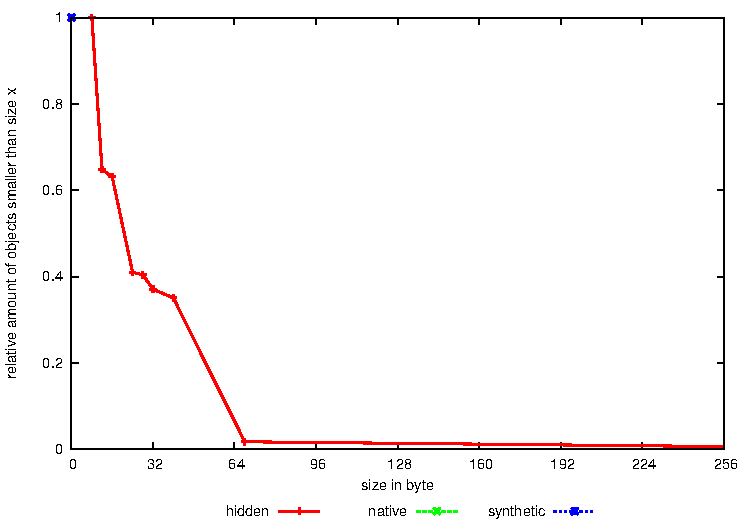
\includegraphics[width=0.5\textwidth]{obj_sys_selfsize_dist}
	\caption{Size distribution of real web applications.}
	\label{fig:obj_sys_selfsize_dist}
\end{figure}

In Figure \ref{fig:obj_sys_lieftiem_dist} we present the lifetime distribution over all snapshots of all workloads separated by the object type. The x-axis show the object lifetime in allocated KB. We decided to use this metric to get rid of the lifetime in snapshots representation. The sample rate of the snapshot generation is 4KB of allocated memory and this leads to an minimum lifetime of 4KB. The lifetime of hidden classes shows a similar behavior than the lifetime of mutator objects of type object as explained in section \ref{sec:analysis_mutator}, especially Figure \ref{fig:obj_lifetime_dist} on page \pageref{fig:obj_lifetime_dist} illustrates. 

\begin{figure}
	\centering
	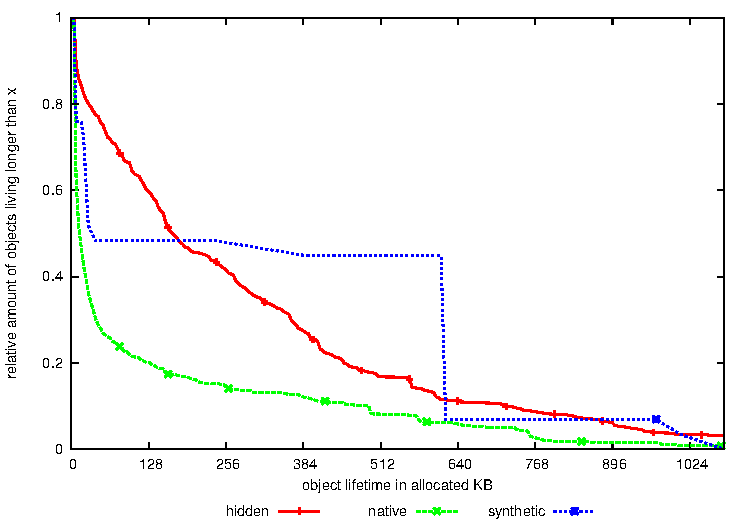
\includegraphics[width=0.5\textwidth]{obj_sys_lifetime_dist}
	\caption{Lifetime distribution of real web applications.}
	\label{fig:obj_sys_lieftiem_dist}
\end{figure}

The root distance of nodes in a graph is an interesting parameter of the graph characteristic. If we look at the root distance of system objects we are faced with some special cases, because objects of type synthetic represent GC roots which are used to compute the root distance, but it is possible that a object of type synthetic also as a GC root. So the root distance of synthetic objects is always zero or one. Objects of type native show a similar behavior because the are also used to represent DOM roots. Nevertheless, the behavior of objects of type hidden provides interesting informations. The Figure \ref{fig:obj_sys_rootdist_dist} illustrates the root distance of the system objects. On the x-axis of the Figure shows the minimum root distance and on the y-axis the relative amount of objects with a root distance smaller than x. This Figure shows that hidden classes have a small root distance and that there are only few objects with a higher root distance.

\begin{figure}
	\centering
	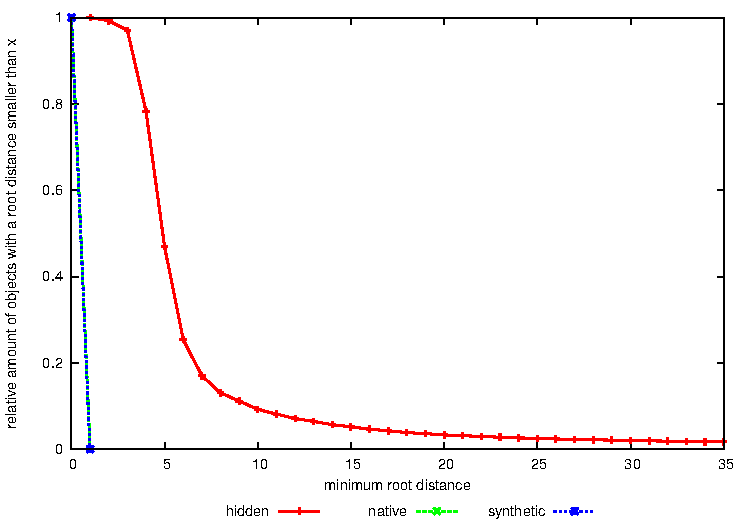
\includegraphics[width=0.5\textwidth]{obj_sys_rootdist_dist}
	\caption{Root distance distribution of real web applications.}
	\label{fig:obj_sys_rootdist_dist}
\end{figure}

The Figure \ref{fig:obj_sys_outdeg_dist} presents the distribution of outgoing edges of a node, the so-called out-degree. This illustration shows the results computed over all snapshots of all workloads. In this Figure we see that objects of type hidden have a out-degree of less than ten. If we have a look at the native line, we recognize that this kind of objects have a significantly higher out-degree than objects of type hidden. Especially objects of type synthetic have a extreme high out-degree, because they represent the GC root and we conclude the heap tree is very breadth.   

\begin{figure}
	\centering
	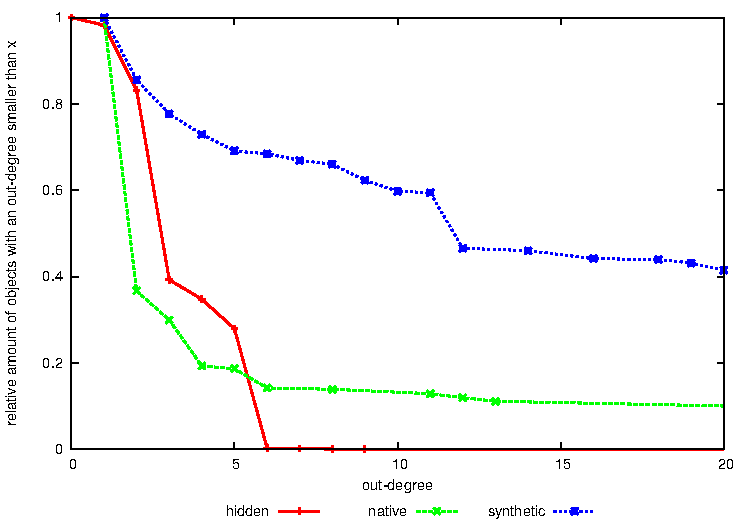
\includegraphics[width=0.5\textwidth]{obj_sys_outdeg_dist}
	\caption{Out-degree distribution of real web applications.}
	\label{fig:obj_sys_outdeg_dist}
\end{figure}

% \begin{figure}
% 	\centering
% 	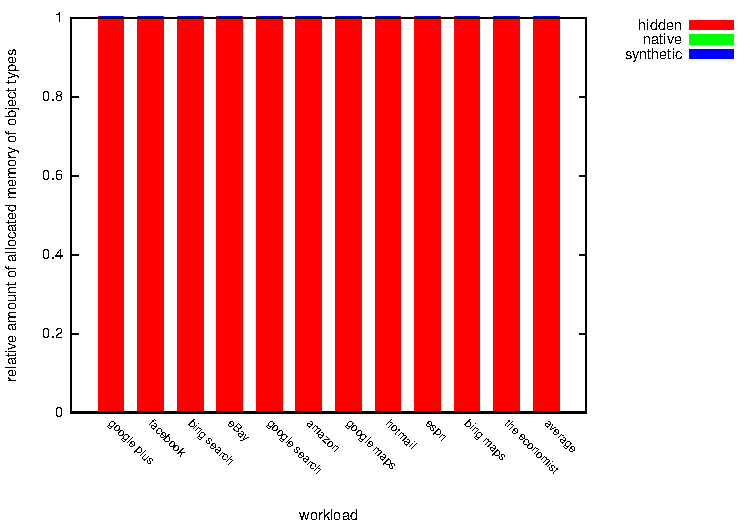
\includegraphics[width=0.5\textwidth]{obj_sys_byte_dist}
% 	\caption{Histogram of the object type distribution for all workloads.}
% 	\label{fig:obj_sys_byte_dist}
% \end{figure}
% 
% \begin{figure}
% 	\centering
% 	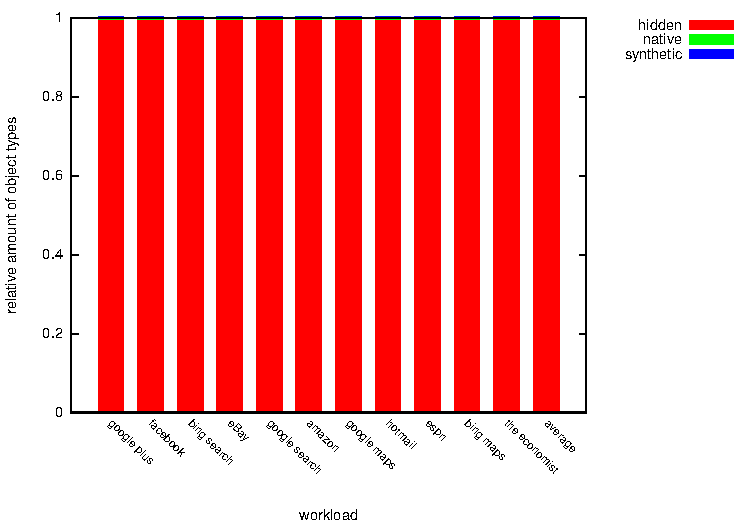
\includegraphics[width=0.5\textwidth]{obj_sys_alloc_dist}
% 	\caption{Histogram of the object type distribution for all workloads.}
% 	\label{fig:obj_sys_alloc_dist}
% \end{figure}
